\chapter{Szenario}
Im Landwirtschaftsbetrieb in Fuchshain wird ein Kühlsystem verwendet, um die Milch auf die richtige Temperatur zu kühlen. Dabei gelangt die gewonne Milch in einen Milchtank, welche dann heruntergekühlt wird. In den eigentlichen Kühlvorgang kann nicht eingegriffen werden, weswegen die Vorkühlung der Milch vor dem Milchtank durch den Eiswasserspeicher gekühlt werden muss. Dieser Eiswasserspeicher soll durch eine vorhandene PV Anlage gespeist werden.\\
Während der Produktion muss die Milch von 35 auf 4 Grad Celsius abgekühlt werden. Diese Kühlmaßname ist energieaufwändig (304342,5 kJ bei 2500 Liter Milch). Damit die Hauptkühlung entlastet werden kann, soll die Effizienz einer Vorkühlung durch einen Eiswasserspeicher ermittelt werden. Dieser Speicher würde eine Abflachung der Lastspitzen ermöglichen und somit dem Betrieb Geld einsparen. Da die Anschaffung eines Eiswasserspeichers kostspielig ist, soll vorerst durch eine SImulation die Rentabilität ermittelt werden. Dabei wird angenommen, dass eine Vorkühlung der Milch von 35 auf 17 Grad Celsius stattfindet.

\section{Eiswasserspeicher}
Der Eiswasserspeicher kann 164 kg Eis speichern. Er verfügt weiterhin über einen Kompressor der Marke Maneurop MT-22 mit 3,51 kW Leistung. Der Kompressor ist für die Erzeugung des Eises verantwortlich. Weiterhin befindet sich im Speicher die horzontale Kreiselpumpe CEA 70/3/A-V der Firma LOWARA. Die Ladezeit für eine komplette Beladung mit Eis wird mit sechs Stunden angegeben.\\
Abbildung \ref{verbrauch1feb} zeigt den Verbrauch der Anlage am 1. Februar 2015 ohne den Betrieb eines Eiswasserspeichers. Die zwei hohen Ausschläge gibt die Leistung der zwei Kühlanlagen wieder. Diese Last soll durch einen Eiswasserspeicher gemindert werden, indem eine Vorkühlung stattfindet. In Kombination mit der PV Anlage erzeugt der Eiswasserspeicher Kühlleistung, welche die eigentliche Last der Hauptkühlung mindern soll.
 \begin{figure}[H]
 	\centering
 	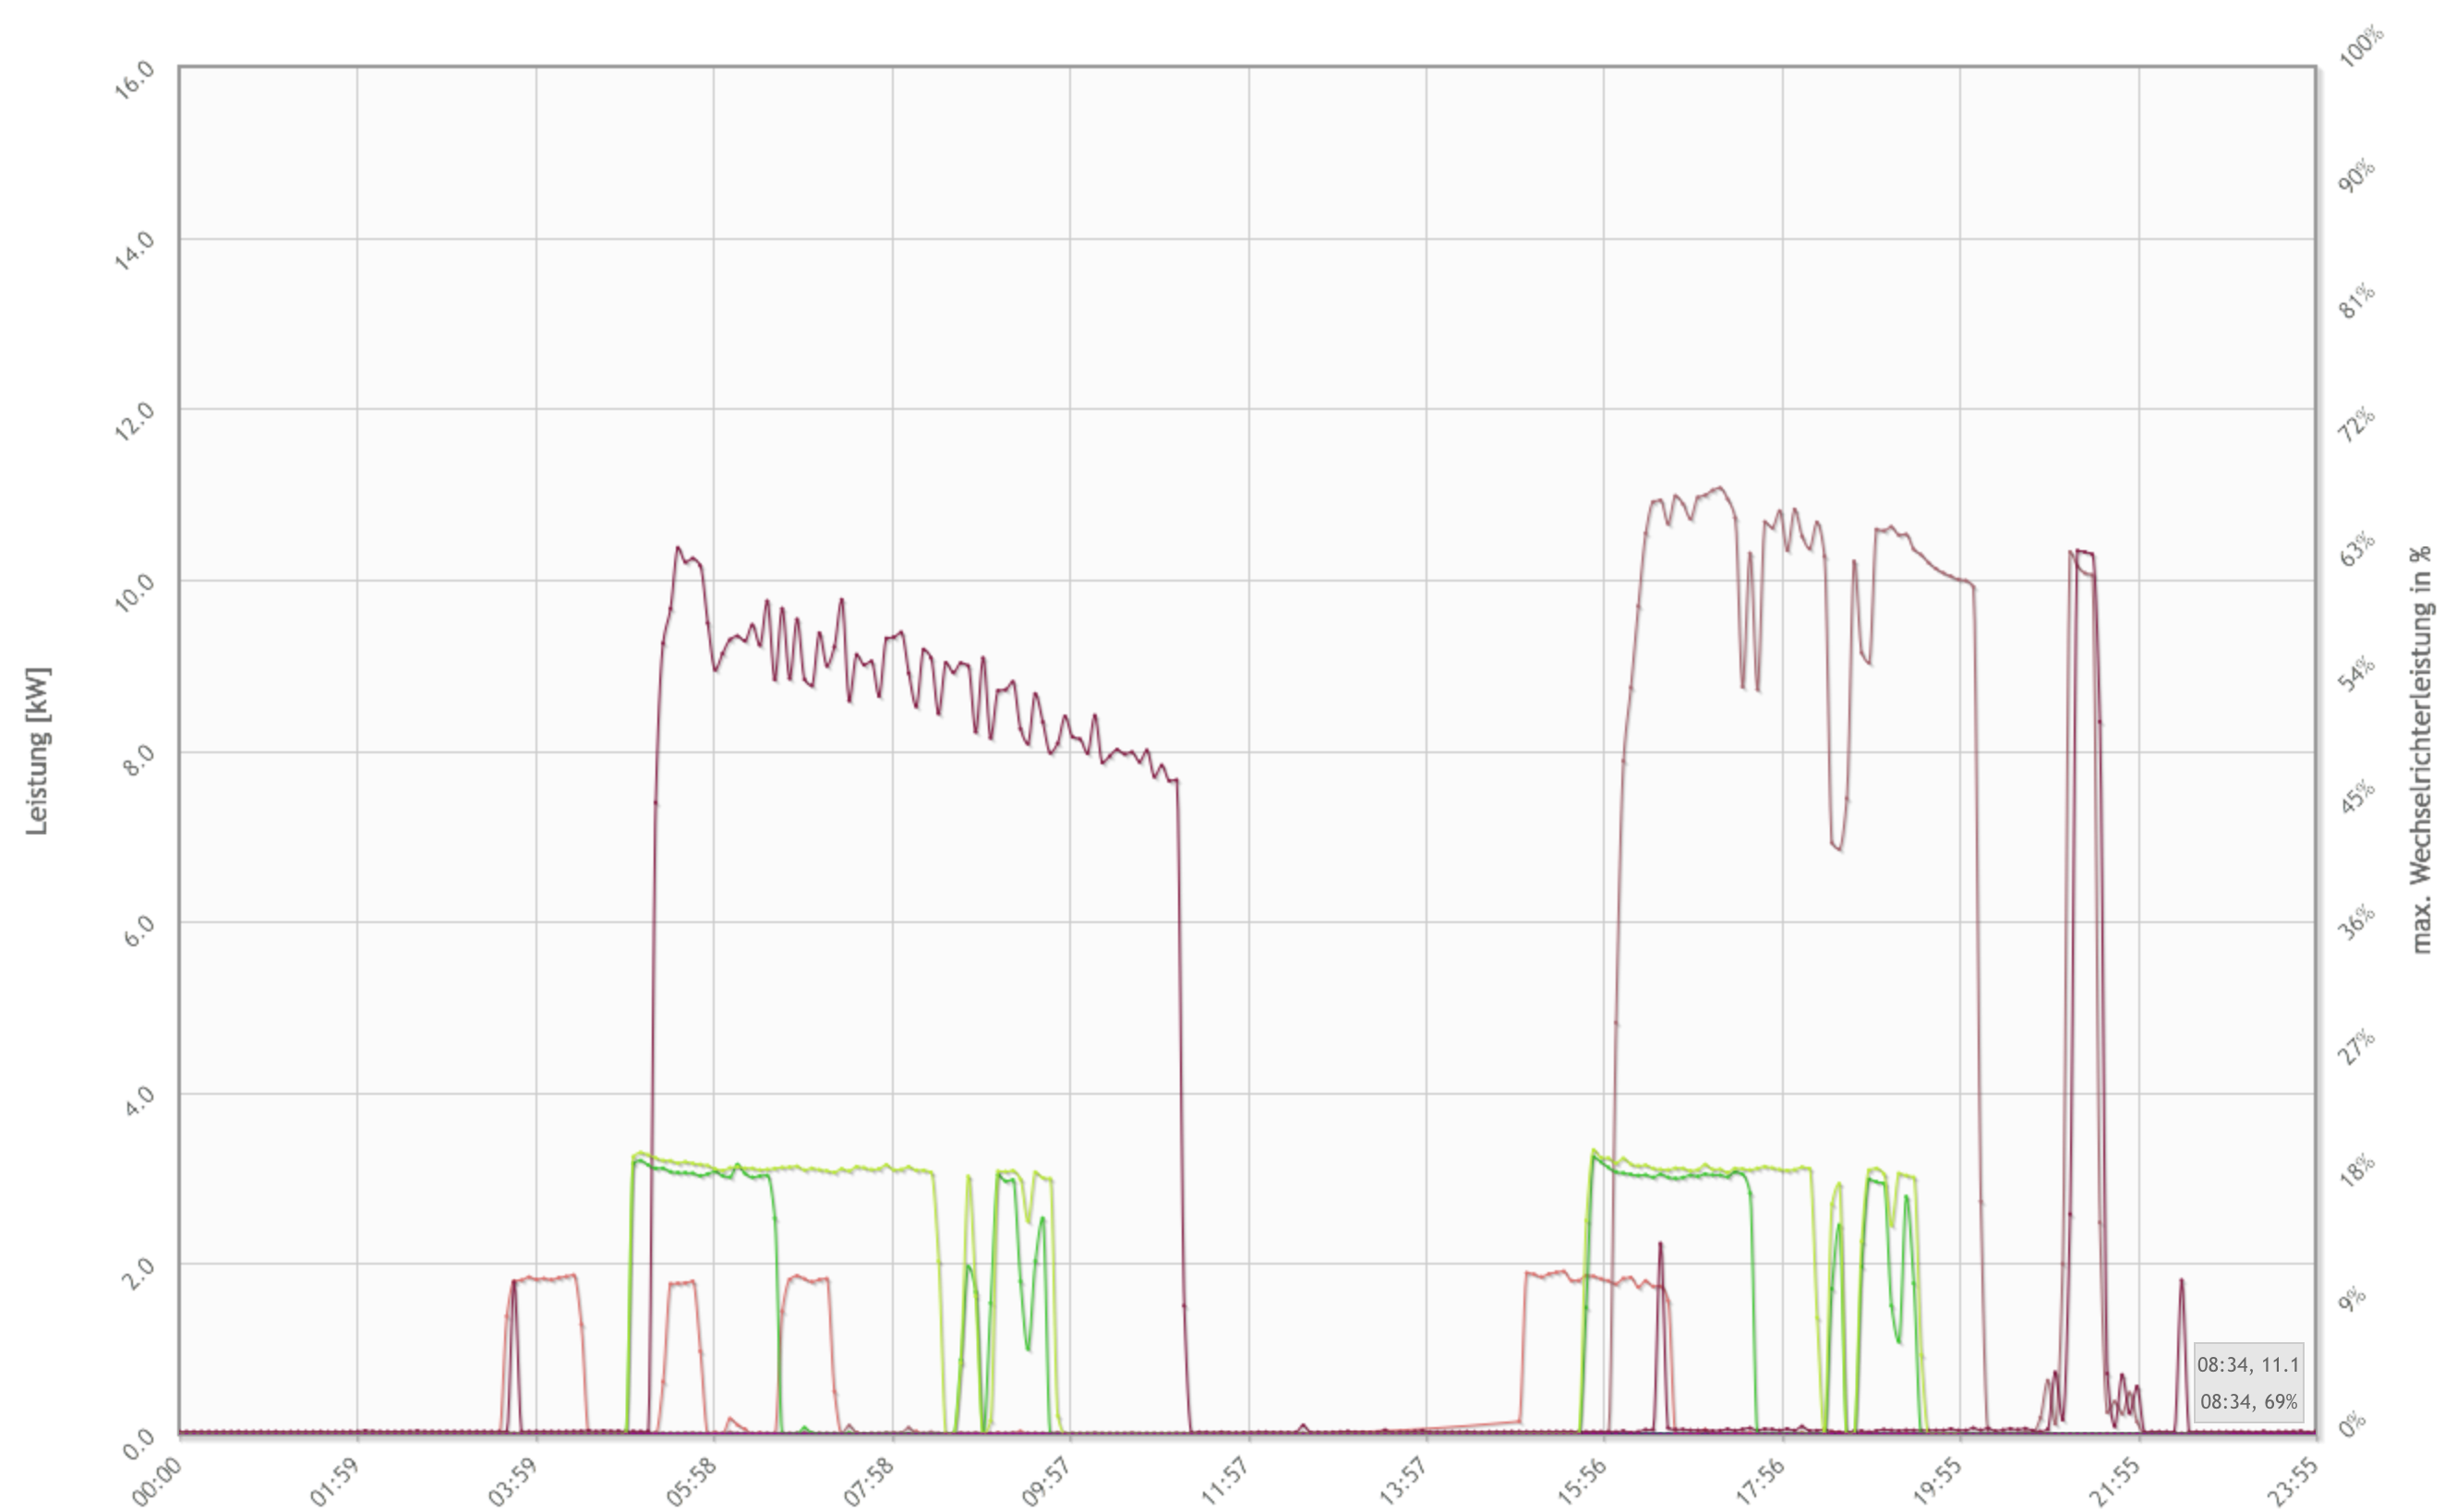
\includegraphics[width=0.8\textwidth]{bilder/verbrauch1feb.png}
 	\caption{Verbrauch 1. Februar 2015}
 	\label{verbrauch1feb}
 \end{figure}

\section{Lösung}
Für die Realisierung des Simulators wurde ein Raspberry PI zur Verfügung gestellt. Dieser soll softwareseitig alle 15 Minuten einen Simulationsschritt durchführen. In einem Schritt wird festgestellt, ob der Speicher beladen oder entladen wird. Während den Schritten wird die benötigte Leistung anhand einer S0-Schnittstelle übertragen. Die Leistung für den Ent- und Beladevorgang wurden vorgegeben.\\
Die S0-Schnittstelle ist nach DIN EN 62053-31 spezifiziert und dient zur Übertragung von Verbrauchsmesswerten. Häufiger Einsatz ist die Gebäudeautomatisierung und findet in einer vielzahl von Messgeräten anwendung. Elektrische Impulse dienen als Maßeinheit für den Verbrauch eines Geräts. Diese Impulse müssen ein gewissen Muster aufweisen, damit sie als gültiger Impuls gewertet werden. Ein Impuls besteht aus einem High und Low Signal. High muss ebenso wie Low mindestens 30 Millisekunden lang sein und die auf bzw. absteigende Flanke muss kleiner als fünf Millisekunden sein. Weiterhin entsprechen 1000 Impulse die Leistung von 1000 Watt.